%% file: template.tex = LaTeX template for article-like report 
%% init: sometime 1993
%% last: Feb  8 2015  Rob Rutten  Deil
%% site: http://www.staff.science.uu.nl/~rutte101/rrweb/rjr-edu/manuals/student-report/

%% First read ``latex-bibtex-simple-manual.txt'' at
%% http://www.staff.science.uu.nl/~rutte101/Report_recipe.html

%% Start your report production by copying this file into your XXXX.tex.
%% Small changes to the header part will make it an A&A or ApJ manuscript.

%%%%%%%%%%%%%%%%%%%%%%%%%%%%%%%%%%%%%%%%%%%%%%%%%%%%%%%%%%%%%%%%%%%%%%%%%%%%
\documentclass{aa}   %% Astronomy & Astrophysics style class

\usepackage{graphicx,natbib,url,twoopt}
\usepackage[varg]{txfonts}           %% A&A font choice
\usepackage{hyperref}                %% for pdflatex
%%\usepackage[breaklinks]{hyperref}  %% for latex+dvips
%%\usepackage{breakurl}              %% for latex+dvips
\usepackage{pdfcomment}              %% for popup acronym meanings
\usepackage{acronym}                 %% for popup acronym meanings

\hypersetup{
  colorlinks=true,   %% links colored instead of frames
  urlcolor=blue,     %% external hyperlinks
  linkcolor=red,     %% internal latex links (eg Fig)
}

\bibpunct{(}{)}{;}{a}{}{,}    %% natbib cite format used by A&A and ApJ

\pagestyle{plain}   %% undo the fancy A&A pagestyle 

%% Add commands to add a note or link to a reference
\makeatletter
\newcommand{\bibnote}[2]{\@namedef{#1note}{#2}}
\newcommand{\biblink}[2]{\@namedef{#1link}{#2}}
\makeatother

%% Commands to make citations ADS clickers and to add such also to refs
%% May 2014: they give error stops ("Illegal parameter number ..."}
%%   for plain latex with TeX Live 2013; the ad-hoc fixes added below let
%%   latex continue instead of stop within these commands.
%%   Please let me know if you know a better fix!
%%   No such problem when using pdflatex.
\makeatletter
 \newcommandtwoopt{\citeads}[3][][]{%
   \nonstopmode%              %% fix to not stop at error message in latex
   \href{http://adsabs.harvard.edu/abs/#3}%
        {\def\hyper@linkstart##1##2{}%
         \let\hyper@linkend\@empty\citealp[#1][#2]{#3}}%   %% Rutten, 2000
   \biblink{#3}{\href{http://adsabs.harvard.edu/abs/#3}{ADS}}%
   \errorstopmode}            %% fix to resume stopping at error messages 
 \newcommandtwoopt{\citepads}[3][][]{%
   \nonstopmode%              %% fix to not stop at error message in latex
   \href{http://adsabs.harvard.edu/abs/#3}%
        {\def\hyper@linkstart##1##2{}%
         \let\hyper@linkend\@empty\citep[#1][#2]{#3}}%     %% (Rutten 2000)
   \biblink{#3}{\href{http://adsabs.harvard.edu/abs/#3}{ADS}}%
   \errorstopmode}            %% fix to resume stopping at error messages
 \newcommandtwoopt{\citetads}[3][][]{%
   \nonstopmode%              %% fix to not stop at error message in latex
   \href{http://adsabs.harvard.edu/abs/#3}%
        {\def\hyper@linkstart##1##2{}%
         \let\hyper@linkend\@empty\citet[#1][#2]{#3}}%     %% Rutten (2000)
   \biblink{#3}{\href{http://adsabs.harvard.edu/abs/#3}{ADS}}%
   \errorstopmode}            %% fix to resume stopping at error messages 
 \newcommandtwoopt{\citeyearads}[3][][]{%
   \nonstopmode%              %% fix to not stop at error message in latex
   \href{http://adsabs.harvard.edu/abs/#3}%
        {\def\hyper@linkstart##1##2{}%
         \let\hyper@linkend\@empty\citeyear[#1][#2]{#3}}%  %% 2000
   \biblink{#3}{\href{http://adsabs.harvard.edu/abs/#3}{ADS}}%
   \errorstopmode}            %% fix to resume stopping at error messages 
\makeatother

%% Acronyms
\newacro{ADS}{Astrophysics Data System}
\newacro{NLTE}{non-local thermodynamic equilibrium}
\newacro{NASA}{National Aeronautics and Space Administration}

%% Add popups with meaning to acronyms 
%% NB: only show up in Adobe Reader and do not work with \input or \include
\gdef\acp#1{%
  \pdfmarkupcomment[markup=Underline,color={1 1 1},author={{#1}},opacity=0]%
  {{#1}}{{\acl{#1}}}}

%% Spectral species
\def\MgI{\ion{Mg}{I}}          %% A&A; for aastex use \def\MgI{\ion{Mg}{1}} 
\def\MgII{\ion{Mg}{II}}        %% A&A; for aastex use \def\MgII{\ion{Mg}{2}} 

%% Hyphenation
\hyphenation{Schrij-ver}       %% Dutch ij is a single character

%%%%%%%%%%%%%%%%%%%%%%%%%%%%%%%%%%%%%%%%%%%%%%%%%%%%%%%%%%%%%%%%%%%%%%%%%%%%
\begin{document}  

%% simple header.  Change into A&A or ApJ commands for those journals

\twocolumn[{%
\vspace*{4ex}
\begin{center}
  {\Large \bf Stellar Spectra A. Basic Line Formation}\\[4ex]       
  {\large \bf Andreas Ellewsen$^{1}$}\\[4ex]
  \begin{minipage}[t]{15cm}
        $^1$ Institute of theoretical astrophysics\\

  {\bf Abstract.} We learned how to write nice reports \ldots 

  \vspace*{2ex}
  \end{minipage}
\end{center}
}] 

%%%%%%%%%%%%%%%%%%%%%%%%%%%%%%%%%%%%%%%%%%%%%%%%%%%%%%%%%%%%%%%%%%%%%%%%%%%%
\section{Introduction}   \label{sec:Intro}
%%%%%%%%%%%%%%%%%%%%%%%%%%%%%%%%%%%%%%%%%%%%%%%%%%%%%%%%%%%%%%%%%%%%%%%%%%%%
This is the first of three numerical exercises in the course on Radiative processes in astrophysics (AST4310) at the University of Oslo. In this exercise we are to follow the steps of Annie Cannon, Cecilia Payne, and Marcel Minnaert. By doing this we hope to learn about the use of spectral lines in astophysics. 


%%%%%%%%%%%%%%%%%%%%%%%%%%%%%%%%%%%%%%%%%%%%%%%%%%%%%%%%%%%%%%%%%%%%%%%%%%%%
\section{Spectral Classification}    \label{sec:Specclas}
%%%%%%%%%%%%%%%%%%%%%%%%%%%%%%%%%%%%%%%%%%%%%%%%%%%%%%%%%%%%%%%%%%%%%%%%%%%%
The first part of this section deals with learning a little about how IDL functions.
You also make a fuction that adds all the numbers in an array together and gives you the result.
This function already exists in IDL, and is called TOTAL, but we make our own function anyway.
The function is called ADDUP, and looks exactly like the function written in the exercise text.
The function has been tested, and it passes all the test I've tried throwing at it (except of course those it will clearly fail, like strings).

The second part of this section deals with LaTeX and gives instructions on how to write a good report.
Basically one is given a template and told a long list of things that are useful to know when writing reports, and then you use this knowledge for the rest of the exercise.

%% {fig:XX}
%===========================================================================
%\begin{figure}[hbtp]
%  \centering
%  \includegraphics[width=80mm]{XX}
%  \caption[]{\label{fig:XX}
%    Caption text \dots
%  }
%\end{figure}
%===========================================================================


%%%%%%%%%%%%%%%%%%%%%%%%%%%%%%%%%%%%%%%%%%%%%%%%%%%%%%%%%%%%%%%%%%%%%%%%%%%%
\section{Saha-Boltzmann calibration of the Harvard sequence}   \label{sec:Saha}
%%%%%%%%%%%%%%%%%%%%%%%%%%%%%%%%%%%%%%%%%%%%%%%%%%%%%%%%%%%%%%%%%%%%%%%%%%%%
Here we want to explain the spectral-type sequence that was studied in the two first parts of the last section (which we ignored).
To start of we study figures 5 and 7 in the exercise text. Starting from the right of figure 5 one sees that the $H\beta$ line lies between $4762 \AA$ and $4954 \AA$. If one looks at figure 7 one sees that the only line between these two wavelengths is the Balmer $\beta$ line at $4861 \AA$. The Balmer $\beta$ line is the transition between $n = 4$ and $n = 2$. 
Considering that the spectrum we're looking at in figure 5 ranges between $3900 \AA$ and $5000 \AA$, which is in the visual part of the spectrum, the rest of the lines corresponding to hydrogen should all be in the Balmer series as well. This means that none of the lines share the same upper level, and that they all share the same lower level, namely $n = 2$.
This is the case for all of these named series. Sharing of the upper levels is a bit more complicated. If one looks at figure 7 one sees that Lyman $\alpha$ shares no upper level with anything. But Lyman $\beta$ shares the same upper level as Balmer $\alpha$. Figure 7 skips some of the transitions. But Lyman $\gamma$ shares upper level with Balmer $\beta$ and Paschen $\alpha$. It keeps going in this way for the rest of the transitions.

At this point Payne made the assumption that the strength of the absorption lines observed in stellar spectra scaled with the population density of the lower level of the corresponding transition. 
This seems logical if one also assumes that most of the hydrogen was in the ground state to begin with.

It turns out that this assumption assumption is not correct, but in general it is true that stellar absorption lines get stronger at larger lower-level population. 

We ignore this and continue with Payne's assumption anyway.

\begin{itemize}
 \item 
Use this expectation to give initial rough estimates of the strength ratios of the $\alpha$ lines in the the H I Lyman, Balmer, Paschen and Brackett series.
\end{itemize}

The Boltzmann distribution is defined
\begin{equation}
\frac{n_{r,s}}{N_r} = \frac{g_{r,s}}{U_r} e^{-\chi_{r,s}/kT} 
\end{equation}


The partition function $U_r$ is define as
\begin{equation}
 U_r = \sum_s g_{r,s} e^{-\chi_{r,s}/kT}
\end{equation}


The Saha law reads
\begin{equation}
 \frac{N_{r+1}}{N_r} = \frac{1}{N_e}\frac{2U_{r+1}}{U_r}\bigg(\frac{2\pi m_e kT}{h^2}\bigg)^{3/2} e^-{\chi_r/kT}.
\end{equation}

\begin{itemize}
 \item 
 Note in the first table that the partition functions computed from (2) are of order unity and barely sensitive to temperature.
\item
In the second table, note the steep Boltzmann population decay with $\chi_{r,s}$ given by (1). It is less steep for higher temperature. The columns add up to unit y because the values in this table are scaled by $N_r$. They therefore depend on $U_r$, but the small variation between $U_1$ and $U_4$ in the first table produces a difference at two-digit significance only for $s = 1$ at $20 000 K$. The partition function $U_1$ of the neutral stage is the sum of only seven levels; the higher levels present in stages $r \ge 2$ contribute only marginally. The ground state always has the largest population.
\item
Inspect the third table, computed from (3). There are only two ionization stages significantly present per column. For T = 5000 K element E is predominantly neutral, for T = 10 000 K it is once ionized ($E^+$), for higher temperature stages $E^{2+}$ and $E^{3+}$ appear while $E$ and $E^+$ vanish.
\item
Explain from (1) and (3) why the Saha and Boltzmann distributions behave differently for increasing temperature.
\item
Speculate why ionization can fully deplete a stage even though excitation puts only a few atoms in levels below the ionization level. Hint: what parameter in the Saha distribution can cause equality between high-level and next-ion population at a given temperature?
\end{itemize}
\subsection{Saha-Boltzmann population of Shadeenium}
Now it is time to reproduce Shadee's tables. This is done by using python routines to compute $U_r$ from (2) and $n_{r,s}/N_r$ from (1), and $N_r/N$ from (3) for element E. All computations are done using cgs units.
%See Fig.~\ref{fig:XX}.
%%%%%%%%%%%%%%%%%%%%%%%%%%%%%%%%%%%%%%%%%%%%%%%%%%%%%%%%%%%%%%%%%%%%%%%%%%%%
\section{Fraunhofer line strengths and the curve of growth}   \label{sec:Fraunhofer}
%%%%%%%%%%%%%%%%%%%%%%%%%%%%%%%%%%%%%%%%%%%%%%%%%%%%%%%%%%%%%%%%%%%%%%%%%%%%
The modeling of \dots

\subsection{Radiation through an isothermal layer}
It can be shown that the total emergent radiation from a layer with optical thickness $\tau(x)$ and temperature $T(x)$ is:
\begin{equation}\label{Radiation_general}
\begin{aligned}
 I_{\lambda} =& I_{\lambda}(0)e^{-\tau} + \int_0^\tau B_{\lambda}[T(x)]e^{-(\tau - \tau(x))}d\tau(x)
\end{aligned}
\end{equation}
If one assumes that the layer is isothermal, this implies that the optical thickness and temperature is independent of position inside the layer. Inserting this into equation \ref{Radiation_general} gives the following

\begin{equation*}
\begin{aligned}
I_{\lambda} =& I_{\lambda}(0)e^{-\tau} + \int_0^\tau B_{\lambda}[T(x)]e^{-(\tau - \tau(x)')}d\tau(x)'\\
	    =& I_{\lambda}(0)e^{-\tau} + B_{\lambda}(T)e^{-\tau}\int_0^\tau e^{\tau'}d\tau'\\
	    =& I_{\lambda}(0)e^{-\tau} + B_{\lambda}(T)e^{-\tau}(e^{\tau} - 1)\\
\end{aligned}
\end{equation*}

\begin{equation}\label{Radiation_isothermal}
 I_{\lambda} = I_{\lambda}(0)e^{-\tau} + B_{\lambda}(1 - e^{-\tau})
\end{equation}

\begin{figure}
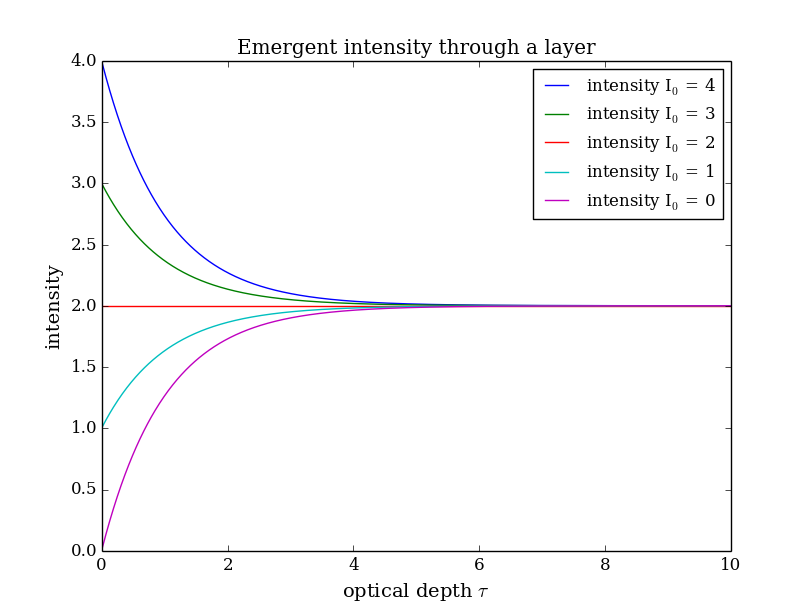
\includegraphics[width=.49\textwidth]{emergent_original.png}
\caption{As the optical depth increases, the intensity converges to the intensity of the Source function B.}
\label{emergent_original}
\end{figure}

\begin{figure}
 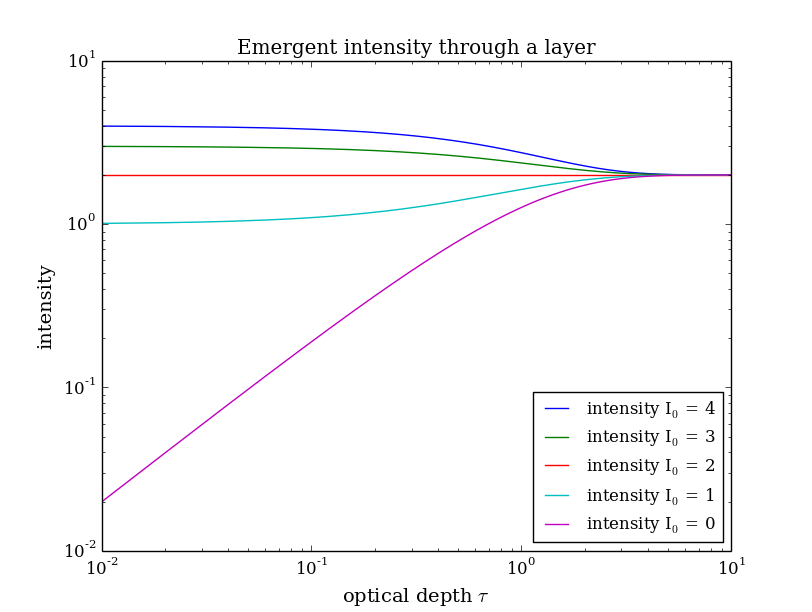
\includegraphics[width=.49\textwidth]{emergent_log.png}
 \caption{The emergent intensity with a logarthimic scale.}
 \label{emergent_log}
\end{figure}
Studying figures \ref{emergent_original} \& \ref{emergent_log} shows a few different things.
If one first considers cases where $tau << 1$, the figures show that if $I_\lambda(0) = 0$, you get an exponential growth due to the source function B. And if $I_\lambda(0) > B_\lambda$ the intensity stays constant. This case corresponds to an ``optically thin'' medium. This is because whatever intensity that enters the medium passes straight through without being affected by the medium.

The opposite case where $\tau >> 1$ is called an ``optically'' thick medium, since all the incident radiation is absorbed before it is able to pass through, and is replaced by the radiation emitted by the medium itself. As seen in the plot, the emergent intensity becomes independent of optical depth for large $\tau$. Mathematically one can see it by looking at equation \ref{Radiation_isothermal} and letting $\tau \rightarrow \infty$. In physical terms one can picture it such that both the incident radiation and the radiation emitted by the medium is absorbed while it is passing through the medium, but since the medium replenishes the radiation it is emitting along the path through it, this radiation is refilled as one goes through the medium.

From this it should be clear that optically thin mediums allow us to view radiation originating from the other side of the medium, while optically thick mediums absorb all of the incident radiation before it can pass through, thus blocking our view past them.

%%%%%%%%%%%%%%%%%%%%%%%%%%%%%%%%%%%%%%%%%%%%%%%%%%%%%%%%%%%%%%%%%%%%%%%%%%%%
\section{Conclusions} \label{sec:conclusions}
%%%%%%%%%%%%%%%%%%%%%%%%%%%%%%%%%%%%%%%%%%%%%%%%%%%%%%%%%%%%%%%%%%%%%%%%%%%%
insert conclusions
%%%%%%%%%%%%%%%%%%%%%%%%%%%%%%%%%%%%%%%%%%%%%%%%%%%%%%%%%%%%%%%%%%%%%%%%%%%%
\begin{acknowledgements}
\end{acknowledgements}

%%%%%%%%%%%%%%%%%%%%%%%%%%%%%%%%%%%%%%%%%%%%%%%%%%%%%%%%%%%%%%%%%%%%%%%%%%%%
%% references
\bibliographystyle{aa-note} %% aa.bst but adding links and notes to references
%%\raggedright              %% only for adsaa with dvips, not for pdflatex
%\bibliography{XXX}          %% XXX.bib = your Bibtex entries copied from ADS

\end{document}


